

\documentclass[a4paper,12pt]{article} % тип документа
\usepackage[margin=1in]{geometry}

% report, book

%  Русский язык

\usepackage[T2A]{fontenc}			% кодировка
\usepackage[utf8]{inputenc}			% кодировка исходного текста
\usepackage[english,russian]{babel}	% локализация и переносы
\usepackage{graphicx}                % Математика
\usepackage{amsmath,amsfonts,amssymb,amsthm,mathtools} 
\usepackage{mathtext}
\usepackage[T2A]{fontenc}
\usepackage[utf8]{inputenc}

\usepackage{wasysym}

%Заговолок
\author{Бичина Марина 
группа Б04-005 1 курса ФЭФМ}
\title{Отчет по лабораторной работе №2.1.6
Эффект Джоуля-Томсона}
\date{\today}


\begin{document} % начало документа

\maketitle
\newpage


\section{Аннотация}
\paragraph{Цель работы:}
1) определить изменения температуры углекислого газа при протекании через малопроницаемую перегородку при разных начльных значениях давления и температуры

2) вычислить по результатам опытов коэффициентов Ван-дер-Ваальса <<a>> и <<b>> \\ \\ \textbf{Оборудование:}
 
1) трубка с пористой перегородкой

2) труба Дьюара

3) термостат

4) термометры

5) дифференциальная термопара

6) микровольтрмер

7) балластный баллон

8) манометр



\section{Теоретическая часть}
\subsection{Теория:}

\paragraph{}	
Эффектом Джоуля–Томсона называется изменение температуры
газа, медленно протекающего из области высокого в область низкого давления в условиях
хорошей тепловой изоляции.
В разреженных газах,
которые приближаются по своим свойствам
к идеальному газу, при таком течении температура газа не меняется. Эффект Джоуля–Томсона демонстрирует отличие исследуемого газа от идеального.

В работе исследуется изменение температуры углекислого газа
при медленном его течении по трубке с пористой перегородкой (рисунок 1). Трубка 1 хорошо теплоизолирована.
Газ из области повышенного давления $P_1$ проходит через множество узких и длинных каналов пористой перегородки 2 в область с атмосферным давлением
$P_2$. Перепад давления $\Delta P = P_1-P_2$ из-за большого сопротивления каналов может быть заметным даже при малой скорости течения газа в трубке. Величина эффекта Джоуля–Томсона определяется по
разности температуры газа до
и после перегородки.

Эффект Джоуля-Томсона характеризуется коэффициентом Джоуля-Томсона, показывающего отношение изменения температуры газа при расширении к изменению давления. Для расчета в работе используется приближенная формула для нахождения коэффициента Джоуля-Томсона для Ван-дер-Ваальсового газа (1)
\begin{equation}
\mu = \dfrac{\Delta T}{\Delta P} \approx \dfrac{\dfrac{2a}{RT}-b}{C_p} 
\end{equation}
где $V$ - молярный объем

$a$ и $b$ - коэффициенты из уравнения Ван-дер-Ваальса

$C_p$ - теплоемкость при постоянном давлении 
\subsection{Описание установки}
 
 \begin{figure}[h]

\centering

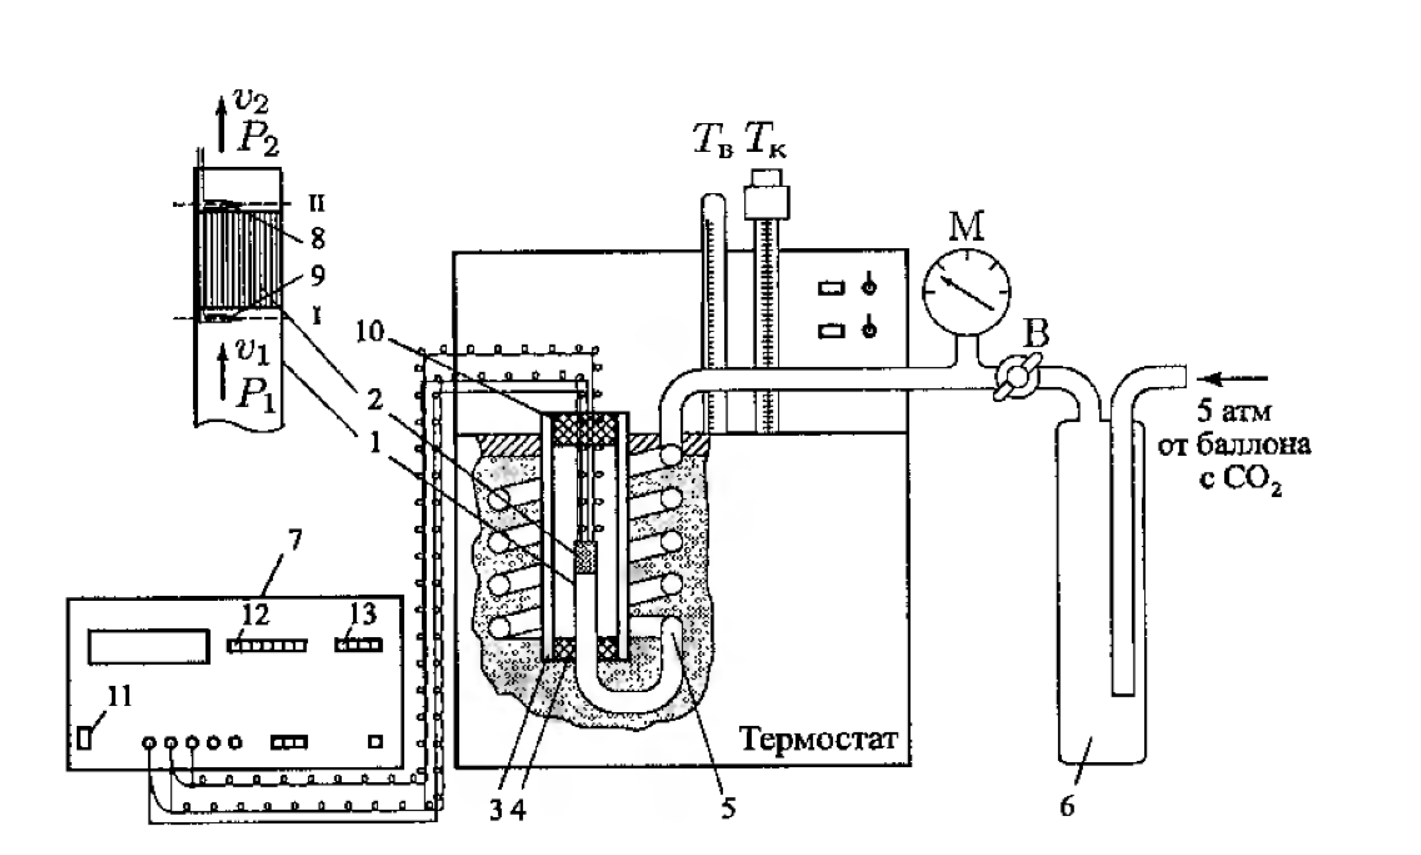
\includegraphics[width=0.8\linewidth]{lab 2.1.6.png}

\caption{Схема установки для изучения эффекта Джоуля-Томсона}

\label{fig:mpr}

\end{figure}


На схеме изображены:\\[0.1 cm]


\begin{minipage}{0.4\textwidth}
  
  1) трубка
  
  2) пористая перегородка
  
  3) трубка Дьюара
  
  4) уплотнение трубки Дьюара кольцом
  
  5) змеевик
  
  6) балластный баллон
\end{minipage}
\hfill
\begin{minipage}{0.4\textwidth}
  
  
  7) цифровой вольтметр
  
  8-9) спаи
  
  10) пробка из пенопласта
  
  11) выключатель <<Сеть>>
  
  12 кнопка <<АВП>>
  
  13 кнопка <<$U_=$>>
  
  
\end{minipage}\\[0.3 cm]

\subsection{Контрольные вопросы:}
\begin{enumerate}
\itemsep0em
\item Чем реальные газы отличаются от идеальных? \\ \\
В модели идеального газа не учитываются притяжение и отталкивание молекул газа между собой (потенциальная энергия). 

В реальных газах молекулы притягиваются на относительно больших расстояниях и отталкиваются вблизи, поэтому уравнение Менделеева-Клапейрона не точно описывает реальный газ и существуют более удачные модели (например, уравнение Ван-дер-Ваальса)

\item Начертите кривые, выражающие характер зависимости сил взаимодействия и взаимной потенциальной энергии двух молекул от расстояния между ними, и, используя их, объясните причины эффекта Джоуля-Томсона\\ \\
\begin{figure}
\begin{minipage}[h]{0.49\linewidth}
\center{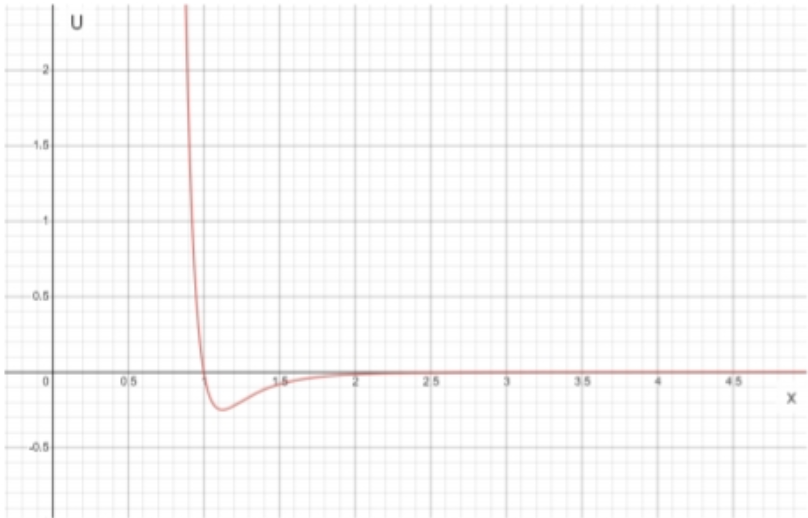
\includegraphics[width=0.7\linewidth]{lenard.png} \\ а)}
\end{minipage}
\hfill
\begin{minipage}[h]{0.49\linewidth}
\center{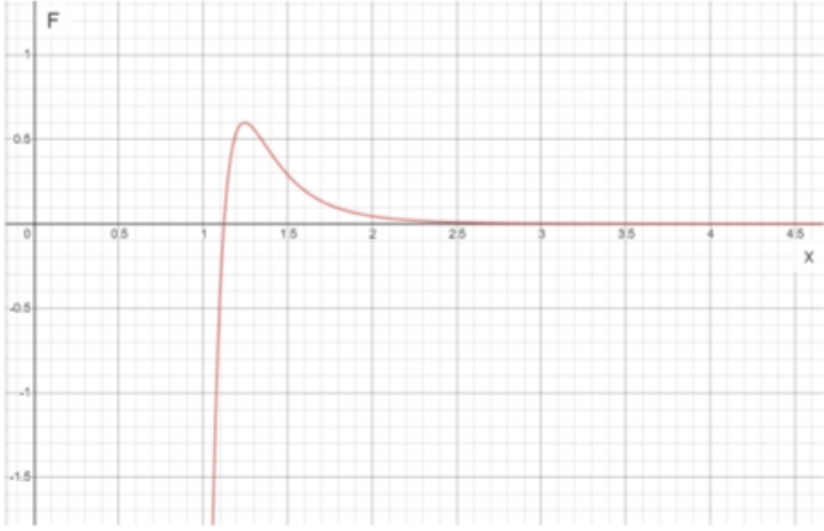
\includegraphics[width=0.7\linewidth]{potential.png} \\ б)}
\end{minipage}
\caption{а) -- Потенциал Леннарда-Джонса, б) -- Зависимость силы от расстояния между молекулами}
\label{ris:image1}
\end{figure}

В эффекте Джоуля-Томсона при идеальном газе  не изменяется температура, но при изменении объема реального газа влияет потенциальная энергия взаимодействия молекул между собой. Изменяется расстояние между молекулами и часть потенциальной энергии взаимодействия молекул переходит в энергию теплового движения и наоборот, то есть в температуру, которая изменяется (но, вроде, не должна была). 
PS Идеальный газ перешел в реальный

\item Какая температура называется критической? Что такое температура инверсии?\\ \\
Критической называется температура, изотерма которой является граничной между монотонными и волнобразными изотермами. Точка, в которой экстремумы изотерм сливаются
Температура инверсии -- это граничная температура, ниже которой газ охлаждается, а выше нагревается (для дифференциального эффекта Джоуля-Томсона)
\item Объясните качественно знак эффекта Джоуля томсона в случае
 
 1) $a = 0,b \not= 0$
 2) $a \not= 0,b = 0$\\ \\
 1) Газ всегда нагревается, поскольку соотношение всегда $(\Delta T/\Delta P)_H<0$ -- (соотношение $(\frac{\Delta T}{\Delta P})_H=\frac{1}{c_p * (dP/dV)_T}(\frac{bRT}{(V-b)^2}-\frac{2a}{V^2})$ для дифференциального эффекта Джоуля-Томсона)
 
 2)Газ всегда охлаждается, поскольку $(\Delta T/\Delta P)_H>0$
\end{enumerate}

\begin{enumerate}

\item  Физический смысл <<a>>, <<b>> \\ \\
Коэффициент b показывает запрещенный молекулам объем $b \simeq$ 4*(объем молекул в одном моле) = $N_AV_0$, поскольку молекулы -- не материальные точки, а <<шары>> радиуса r. Для эффекта Джоуля-Томсона b -- влияет на нагрев газа. Включает в себя силы отталкивания.

Коэффициент a учитывает притяжение молекул, например, через перераспределение зарядов внутри молекул и образование диполей. Для эффекта Джоуля-Томсона а -- влияет на охлажение газа. 
\item Чем отличается изотерма газа Ван-дер-Ваальса от изотермы реального газа и что описывают их разные участки.\\ \\
В отличие от случая идеального газа, некоторые изотермы газа Ван-дер-Ваальса ведут себя немонотонно. При одном и том же давлении вещество может обладать разным объемом. Для левой части$V < 3b$ -- соизмеримо с размером молекул => жидкость, для правой части $V > 3b$ - газ 

BD может быть реализовано только в неравновесном процессе и не может существовать неограниченно долго, т.к. состояние неустойчиво, поскольку не выполняется $(dP/dV)_T < 0$
\begin{figure}[h]
\center{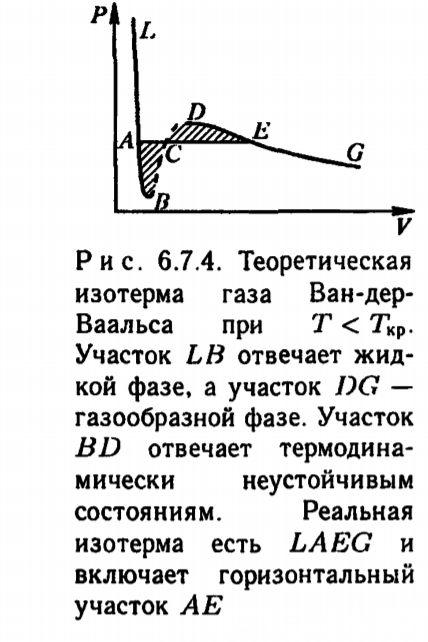
\includegraphics[width=0.36\linewidth]{VDV.png}}
\end{figure}
\item Что такое критическая точка?\\ \\ 
Точка на диаграмме состояния веществ, соответствующая критическому состоянию, то есть конечная точка кривой сосуществования 2 и более фаз 
\item Что такое энтальпия.\\ \\
Энтальпия -- функция состояния термодинамической системы, равная $H = U + PV$. Для идеального газа $H = C_PT$


\end{enumerate}
\section{Экспериментальная часть}
\subsection{Ход работы}
\begin{enumerate} 
\itemsep0em
\item Перед началом работы убедимся в том, что термостат залит водой,
а все электрические приборы заземлены.
\item Установим на контактном термометре $T_k$ температуру регулирования, близкую к комнатной, и включим термостат. 
\item Включим вольтметр. Запишем знак и величину показаний для вольтметра при $\Delta P = 0$. Используем эту величину для корректировки показаний вольтметра в дальнейших измерениях: $E = U(P)-U(0)$.

Откроем регулирующий вентиль настолько, чтобы избыточное давление составило $\Delta P \approx 4$ атм.
\item Через 10–15 минут после подачи давления запишем показания вольтметра
\item При помощи вентиля В установим давление на 0,3–0,5 атм меньше первоначального. Через 5 минут, когда
установятся давление и разность температур, вновь запишите показания манометра и вольтметра. Повторим операцию 5-7 раз для разных значениях давления при комнатной температуре.
\item Построим график зависимости $\Delta T (\Delta P)$ и по наклону определим коэффициент Джоуля-Томсона для выбранной температуры
\item Окончив измерения при комнатной температуре, установим температуру, равную $50 ^oC$. Проделаем действия, аналогичные 3-6. 
\item Проделаем измерения 3-6 для температуры $80 ^oC$
\item Произведем вычисления: найдем <<a>>, <<b>> и $T_{inv}$ для $CO_2$. Сравним их с табличными значениями
\item Обработаем результаты
\item Оценим ошибки измерений 

\end{enumerate}
\subsection{Полученные результаты}
\paragraph{}

Значения для разницы давления даны в больших делениях манометра. На 100 делений манометра приходится 
6 $ \text{кгс} / \text{см}^2 $. Переведём эти значения в атмосферы ($ 1 \text{дел} \approx 0.058 \text{атм} $).
Также разницу потенциалов на термопаре в разницу температуры для каждого измерения и запишем 
 $ \Delta U_i = U_i - U_0 $, где $ i $ - номер измерения.
 Далее осуществим перевод $ \Delta U $ в $ \Delta T $ по соотношению: 
 $ \Delta T = \alpha \Delta U$,
 где $\alpha$ зависит от значения температуры термостата:
\begin{center} 
 \begin{tabular}{|l||l|l|l|}
 \hline 
 T, $^oC$ & 18 & 30 & 50 \\ 
 \hline 
 $\alpha$, мкВ / K & 39,8 & 41,6 & 43,3 \\ 
 \hline 
 \end{tabular}
\end{center} 
 Результаты записаны в таблицах 1, 2 и 3.

\paragraph{Характеристики установки:}
\subparagraph{Систематические погрешности:}
\begin{enumerate}
\itemsep0em
\item Погрешность $ \sigma_{\Delta P} = 0.5 \text{ дел} = 0.03 \text{ атм}$.
\item Погрешность $\sigma_{\Delta U} = 0.001 \text{ мкВ} $ откуда находим погрешность $\sigma_{\Delta T}$, зависящую от температуры.

 Мы используем различные значения коэффициентов для перевода $\Delta U$ в $\Delta T$ при различных температурах термостата, но поскольку значения $\alpha$ отличаются друг от друга не более чем на 5\% возьмём усредненное значение:
\item $\alpha = 39.8 \text{ мкВ/К}$
\item $\sigma_{\Delta T} = 0.05$ K.
\end{enumerate}
\subparagraph{Начальные условия:}
\begin{enumerate}
\itemsep0em
\item Температура термостата: $T_0 = 18^0 C$
\item Напряжение до подачи давления: $U_0 = 0,007$ мВ
\item Давление измеряется в кгс/см$^2$, цена деления -- 0,06 кгс/см$^2$
\end{enumerate}

\textbf{Таблицы с обработанными данными:}
\\ \\
\begin{minipage}{0.5\textwidth}
  \begin{flushleft}

	\begin{tabular}{ | l | l | l | l |}
\hline
N & $\Delta$P,атм &T,$^0C$ & $\Delta$Т,$^0C$ \\ \hline
0 & 0.0 & 18.0 & 0.0 \\
1 & 4.065 & 18.15 & 4.322 \\
2 & 3.717 & 18.23 & 3.894 \\
3 & 3.339 & 18.29 & 3.467 \\
4 & 2.962 & 18.37 & 3.015 \\
5 & 2.671 & 18.45 & 2.663 \\
6 & 1.974 & 18.51 & 1.859 \\
7 & 1.713 & 18.62 & 1.583 \\
\hline
\end{tabular}


Таблица 1 -- данные для комнатной температуры
  \end{flushleft}
\end{minipage}
\begin{minipage}{0.5\textwidth}
  \begin{flushright}
	\begin{tabular}{ | l | l | l | l |}
\hline
N & $\Delta$P,атм &T,$^0C$ & $\Delta$Т,$^0C$ \\ \hline
0 & 0.0 & 30.06 & 0.0 \\
1 & 4.181 & 30.1 & 3.846 \\
2 & 3.862 & 30.08 & 3.462 \\
3 & 3.078 & 30.01 & 2.62 \\
4 & 2.671 & 30.02 & 2.188 \\
5 & 2.584 & 30.0 & 2.115 \\
6 & 2.236 & 30.0 & 1.755 \\
7 & 1.568 & 30.0 & 1.082 \\
\hline
\end{tabular}

 
Таблица 2 -- данные для температуры $\simeq 30$
  \end{flushright}
\end{minipage}

\begin{center}
\begin{tabular}{ |l||l|l|l| } 

\hline
N & $\Delta$P,атм &T,$^0C$ & $\Delta$Т,$^0C$ \\ \hline
0 & 0.0 & 50.0 & 0.0 \\
1 & 4.007 & 50.04 & 2.956 \\
2 & 3.775 & 50.04 & 2.656 \\
3 & 3.339 & 50.01 & 2.286 \\
4 & 2.933 & 50.0 & 1.894 \\
5 & 1.945 & 50.0 & 1.016 \\
 \hline

\end{tabular}
\end{center}
\begin{center}


Таблица 3 -- данные для температуры $\simeq 50$
\end{center}

\paragraph{}
По получившимся значениям для $\Delta P$ и $\Delta T$ построим график зависимости $\Delta T \left( \Delta P \right)$. 
Воспользуемся для аппроксимации методом наименьших квадратов $ y = a_1 + b_1x $:
\[
b_1 = \frac{\langle xy \rangle - \langle x \rangle \langle y \rangle}{\langle x^2 \rangle - \langle x \rangle ^ 2}, \;\;
a_1 = \langle y \rangle - b_1 \langle x \rangle .
\]
Найдём погрешности коэффициентов $a$ и $b$ по формулам:
\[
\sigma_{b_1} \approx \frac{1}{\sqrt{N}}\sqrt{\frac{\langle y^2 \rangle - \langle y \rangle ^ 2}{\langle x^2 \rangle - \langle x \rangle ^ 2} - b_1^2}, \;\;
\sigma_{a_1}  = \sigma_{b_1} \sqrt{\langle x^2 \rangle - \langle x \rangle ^ 2}.
\]
Подставим значения из таблиц 1, 2 и 3. Учтем: $\Delta P \Rightarrow x$ и $\Delta T \Rightarrow y$ \\ \\

\begin{figure}[h]
\center{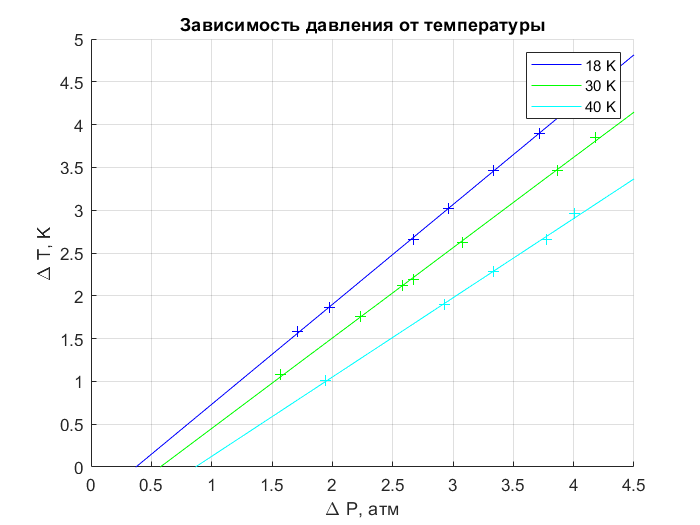
\includegraphics[width=1\linewidth]{plot_1.png}}
\end{figure}
 Полученные значения занесем в таблицу 4:
 
 \begin{table}[h]
\begin{center}
\begin{tabular}{|l||l|l|l|}
\hline 
 & $T =18^oC$ & $T = 30 ^oC$ & $T = 50 ^oC$ \\ 
\hline 
$b_1$, K/атм & 1,167 & 1,06 & 0,93 \\ 
\hline 
$\sigma_{b_1}$, К/атм & 0,006 & 0,01 & 0,02 \\ 
\hline 
$a_1$, К & -0,437 & -0,61 & -0,80 \\ 
\hline 
$\sigma_{a_1}$, К & 0,008 & 0,01 & 0,01 \\ 
\hline 
\end{tabular} 
\end{center}
\begin{center}

Таблица 4 -- Значения полученные 
для $a_1$ и $b_1$

\end{center}
\end{table}
Получим значения для коэффициента Джоуля-Томсона:
\[
\mu_\text{Д-Т} = \frac{\Delta T}{\Delta P} = \frac{A + B \Delta P}{\Delta P} = B + \frac{A}{\Delta P}
\]
Погрешность для $\frac{A}{\Delta P}$: 
\[
\sigma_{A'} = \frac{A}{\Delta P} \sqrt{\left(\frac{\sigma_A}{A}\right)^2 + \left(\frac{\sigma_{\Delta P}}{\Delta P}\right)^2}. 
\]
Диапазон измерений: $ 1,5\text{ атм} < \Delta P < 4,5 \text{ атм} $, значит:
\[
\max{\sigma_{A'}} = \frac{A}{4,5 \text{ атм}} \sqrt{\left(\frac{\sigma_A}{A}\right)^2 + \left(\frac{\sigma_{\Delta P}}{\Delta P}\right)^2}. 
\]
Теперь посчитаем константы Джоуля-Томсона для снятых значений температуры в определённом ранее диапазоне:

Для $T = 18 ^oC$;
\begin{equation*}
 \mu_\text{Д-Т} = 1,167 \pm 0,006 \text{ К/атм} - \frac{0,437 \text{ К}}{\Delta P} \pm 0,002  \text{ К/атм}
\end{equation*}
\paragraph{}
Для $T = 30 ^oC$;
\begin{equation*} 
\mu_\text{Д-Т} = 1,06 \pm 0,01 \text{ К/атм} - \frac{0,61 \text{ К}}{\Delta P} \pm 0,002  \text{ К/атм}
\end{equation*}

\paragraph{}
Для $T = 50 ^oC$;
\begin{equation*}
 \mu_\text{Д-Т} = 0,93 \pm 0,02 \text{ К/атм} - \frac{0,80 \text{ К}}{\Delta P} \pm 0,005  \text{ К/атм}
\end{equation*}

\paragraph{}
Константы Джоуля-Томсона получились зависимыми от разницы давления, поэтому для подсчёта коэффициентов a и b из уравнения Ван-дер-Ваальса используем усреднённое значение коэффициентов Джоуля полученные нами для диапазона давления, рассчитанные по формуле:

\[
\bar{\mu} = \frac{
	\mu_\text{Д-Т}\left( 1,5 \text{ атм} \right) + \mu_\text{Д-Т}\left( 4,5 \text{ атм} \right)}{2}, \;  \sigma_{\bar{\mu}} = \mu_\text{Д-Т}\left( 1,5 \text{ атм} \right) - \bar{\mu}.
\]

\begin{table}[h]	
\begin{center}
\begin{tabular}{|c|c|}
\hline 
T,$^oC$ & $\bar{\mu} \pm \sigma_{\bar{\mu}}$, К/атм \\ 
\hline 
18 & $1,0 \pm 0,2$  \\ 
\hline 
30 & $0,8 \pm 0,3$ \\ 
\hline 
50 & $0,6 \pm  0,4$\\ 
\hline 
\end{tabular} 
\end{center}
\begin{center}

Таблица 5 -- Рассчитанные коэффициенты Джоуля-Томсона

\end{center}
\end{table}

\paragraph{}
На основе полученных значений для коэффициента Джоуля-Томсона рассчитаем коэффициенты Ван-дер-Ваальса по формулам:
\begin{equation*}
b = \frac{C_p \left(T_1 \mu_1 - T_2 \mu_2 \right)}{T_2 - T_1} \\
a = \frac{2 C_p R \left( \mu_1 - \mu_2 \right) }{2 \left( 1/T_1 + 1/T_2 \right)}
\end{equation*}
 Где значения $\mu_1$ и $\mu_2$ можно найти из формул
\begin{equation*} 
\mu_1 = \frac{\frac{2a}{R T_1} - b}{C_p} \\
\mu_2 = \frac{\frac{2a}{R T_2} - b}{C_p}
\end{equation*}

Найдем погрешности для а и b. Заметим, что погрешности $\mu_1$ и $\mu_2$ намного больше погрешностей для значений температуры, поэтому:

\[
\sigma_b = b \frac{\sqrt{T_1^2 \sigma_{\mu_1}^2 + 
T_2^2 \sigma_{\mu_2}^2}}{T_1 \mu_1 - T_2 \mu_2}
\]

\[
\sigma_a = a \frac{\sqrt{\sigma_{\mu_1}^2 + \sigma_{\mu_2}^2}}{\mu_1 - \mu_2}
\]

Подставим в эти формулы значения коэффициента Джоуля-Томсона для разных значений температуры, результат запишем в таблицу 6. Заметим, что погрешности получились весьма большими, что говорит о сложности ведения дальнейший расчетов

\begin{table}
\begin{center}
\begin{tabular}{|l|l|l|l|}
\hline 
$T_1$  $^oC$ & 18 & 30 & 50 \\ 
\hline 
$T_2$ $^oC$ & 30 & 50 & 18 \\ 
\hline  
$a$ & 3592 & 7410 & -3784 \\ 
\hline 
$\sigma_a$ & 2335 & 3705 & 4730 \\ 
\hline 
$b$ & 117 & 88 & 70 \\ 
\hline 
$\sigma_b$ & 261 & 128 & 229 \\ 
\hline 
\end{tabular} 
\end{center}
\begin{center}

Таблица 6 -- Значения коэффициентов a и b

\end{center}
\end{table}

\section{Выводы}
\begin{enumerate}
\itemsep0em
\item Установили линейную зависимость (график 1)  
\item В ходе эксперимента был измерен эффект Джоуля-Томсона. (таблица 4) Константы сильно отличаются от табличных данных. Вероятно, мы не учли некоторые внешние условия, смещающие значения коэффициента Ван-дер-Ваальса, поскольку их отношение сохраняется (по доказанной линейной зависимости) 
\item Получили большую погрешность в измерении коэффициента Джоуля-Томсона. Эти расхождения могут быть объяснены ошибками в проведении эксперимента или проблемами, связанными с самой установкой. 

\end{enumerate}

\end{document} % конец документа